%%This is a very basic article template.
%%There is just one section and two subsections.
\documentclass{article}
\usepackage{amsmath}
\usepackage{amsthm}
\usepackage{amssymb}
\usepackage{listings}
\usepackage[utf8]{inputenc}
\usepackage{graphicx}
\usepackage[hmargin=2.5cm,vmargin=2.5cm]{geometry}
\usepackage[french]{babel}


\usepackage[T1]{fontenc}
\usepackage{uarial}

\renewcommand{\familydefault}{\sfdefault}


\newtheorem{theoreme}{Théorème}[section]
\newtheorem{demonstration}{Démonstration} [section]
\theoremstyle{definition}
\newtheorem{definition}{Définition} [section]



\lstdefinelanguage{JavaScript}{
  morekeywords={typeof, new, true, false, catch, function, return, null, catch, switch, var, if, in, while, do, else, case, break},
  morecomment=[s]{/*}{*/},
  morecomment=[l]//,
  morestring=[b]",
  morestring=[b]',
  frame= single
}

\begin{document}

\begin{titlepage}
\vspace*{.18\textheight}
\begin{center}
%
\begin{figure}[h]
\centering

\includegraphics[scale=0.12]{images/LogoSupelec}
\end{figure}
%
\vspace*{10pt}
\textbf{\LARGE Les ensembles de Julia et de Mandelbrot et les fractales de Newton} \\[0.5 cm]

Gustavo \textbf{CIOTTO PINTON}\\
Luana Ianara \textbf{RUBINI RUIZ}\\
Marcelo \textbf{MARQUES FREIRE DE CARVALHO}\\
Thiago \textbf{AZEVEDO}\\

\vspace*{10pt}
Séquence 5 - Promotion 2013-2015\\[1 cm]

\vspace*{60pt}
Octobre 2014

\end{center}
\end{titlepage}

\section{Ensembles de Julia, Fatou et Mandelbrot}

\subsection{Rappels}

Les ensembles de Julia et de Fatou, notés \(J(f)\) et \(F(f)\) respectivement,
sont définis à partir d'une fonction \(f\). La définition initiale, donnée par
les mathématiciens Pierre Fatou et Gaston Julia, prennait en compte des
fonctions \(f\) rationnelles, mais on peut bien sûr l'étendre à d'autres classes
de fonctions, comme, par exemple, celles dites \textit{holomorphes}. Dans la
suite, on ne traite que le cas particulier des fonctions polynomiales du second
degré et, pour cette raison, on répresente ces ensembles seulement par
\(J\) ou \(F\).

\vspace{12pt}

On commence alors en définissant formallement les deux concepts des ensembles de
Julia et Fatou.

\begin{definition}

Soit \(c \in  \mathbb{C}\) . On appelle \textit{ensemble de Julia rempli de
paramètre} \(c\), \(J_r(c)\), l’ensemble des \(z \in  \mathbb{C}\) tels que la
suite (\(z_n\)) définie par \(z_0 = z \) et \(z_{n+1} = z_n^2 + c \) est bornée (en
module). L’\textbf{ensemble de Julia de paramètre \(c\)}, noté \(J(c)\), est
défini comme la frontière de l’ensemble de Julia rempli de paramètre c.

\end{definition}

\begin{definition}

Soient \(c \in  \mathbb{C}\) et \(J(c)\) son respectif ensemble de Julia de
paramètre \(c\). L'\textbf{ensemble de Fatou} \(F(c)\) est défini comme
l'ensemble complémentaire de \(J(c)\), c'est-à-dire, \(F(c) = J_r(c) - J(c)\).

\end{definition}

En pratique, pour une valeur \(c\) donnée, l'ensemble de Julia correspond aux
points de la frontière de l'ensemble des valeurs initiales \(z_0\) pour
lesquelles la suite est bornée en module, alors que l'ensemble de Fatou
correspond aux points dans son intérieur.

\vspace{12pt}

%En s'appuyant sur ces deux définitions, on peut alors décrire l'ensemble de
%Mandelbrot. Il est défini comme l'ensemble des \(c\) pour lequel son respectif
%\(J(c)\) est connexe, c'est-à-dire que \(c\) appartient à \(M(c)\) si et
%seulement si la suite reste bornée en module. Formellement, on écrit:


%\begin{definition}

%\textbf{L'ensemble de Mandelbrot}, \(M(c)\) est défini comme l'ensemble \(c \in 
%\mathbb{C} \) pour lesquels la suite 
%\[(z_n)_n:\left \{
%   \begin{array}{r c l}
%      z_0  & = & 0 \\
%      z_{n+1}   & = & z_n^2 + c \\
%   \end{array}
%   \right. \]
%reste borné.

%\end{definition}
 
\subsection{Simulation}

\subsubsection{Implémentation}

Avant de donner les détails téchniques sur l'implémentation du programme qui
simule les ensembles décrits ci-dessus, on présente tout d'abord le critère qui
a été utilisé pour déterminer si la suite \((z_n)_n\) converge ou pas. 

\begin{theoreme}

Si la suite des modules des \(z_n\) dépasse 2 pour un certain indice, alors
cette suite est croissante à partir de cet indice, et elle tend vers l'infini.

\end{theoreme}

\begin{demonstration}

Soit \(\alpha\) la racine positive de l'équation \(\alpha^2 = \alpha~ + |c|\)
(donc \(\alpha \geq 1\)). En posant \(x_n = | z_n |  – \alpha\), on a
:
\[\alpha + x_{n+1} \geq (\alpha + x_n)^2 – |c|\]
d'où 
\[x_{n+1} \geq 2\alpha x_n\]
Par conséquent si, pour un certain indice k, \(|z_k| > \alpha\), alors, à
partir de cet indice, la suite \((x_n)\) croît géométriquement.
Ceci a lieu en particulier, pour \(|c| > 2\) dès que k = 1, mais aussi pour
\(|c| \leq 2\), dès que pour un certain k, \(|z_k| > 2\).

\end{demonstration}

En s'appuyant sur ce théorème, on peut alors construire une suite \(z_n\) avec
un nombre fini d'éléments en vérifiant toujours le module de \(z_n\). Si
son module dépasse 2, alors on peut concluire que \(z_n\) n'appartient pas à
l'ensemble de Julia (resp. Mandelbrot). Par contre, si au bout de la n-ème
itération, \(|z_n|\) ne vaut plus que 2, donc on conclut qu'il fait partie de
\(J(c)\) (resp. \(M(c)\)). On a choisi arbitrairement d'itérer jusqu'à
\(n=200\).

\vspace{12pt}

On présente alors la fonction qui vérifie cette condition, implementée en
\textit{JavaScript}.

\newpage

\begin{lstlisting}[language=JavaScript]

function getModule(x, y) {
	
	return Math.sqrt(x*x + y*y);
}

function isJulia(point) {

	var x = 0,
	    un = {a:point.a, b:point.b, module: getModule(point.a, point.b)};
	
	while (x < 200 && un.module < 2) {
		
		var 	x_aux = un.a*un.a - un.b*un.b + c.a,
			y_aux = 2*un.a*un.b + c.b;
			  
		un.a = x_aux;
		un.b = y_aux;
	
		un.module = getModule(x_aux, y_aux);
		x++;
	}

	if (un.module > 2) return x;
	
	return -1;
}
\end{lstlisting}

\vspace{12pt}

On note deux fonctions: la première, \textit{getModule(x,y)}, reçoit deux
valeurs entières (x répresentant \(\operatorname{Re}(z)\) et y,
\(\operatorname{Im}(z)\)) et rétourne leur module, et la deuxième, 
\textit{isJulia(point)} qui itére sur un point reçu comme paramètre et rétourne
soit -1, indiquant que ce point appartient à l'ensemble, soit l'indice d'échec,
qui sera utilisée pour déterminer la couleur du respectif \textit{pixel} qui
répresente ce point. Dans ce dernière fonction, les variables \textit{un} et
\textit{point} sont d'objets qui contiennent les attributs \textit{a},
\textit{b} et \textit{module}, représentant respectivement la partie
réelle, complèxe et le module de chaque point.

\vspace{12pt} 

On remarque encore la fonction suivante, appelée \textit{getPointAsZ}, est
responsable pour transformer les coordonnées \((i,j)\) d'un pixel quelconque en un numéro
complèxe \(z = a+bi\), en considérant toujours  \(\operatorname{Re}(z) \in
[a_{min}, a_{max}]\) et \(\operatorname{Im}(z) \in [b_{min},
b_{max}]\). Les variables \(width\) et \(height\) correpondent aux dimension
d'aire de peinture. Cette transformation consiste à  

\[
\left\{
   \begin{array}{r c l}
      \operatorname{Re}(z) = a = & \frac{i}{width}*(a_{max} - a_{min}) +
      a_{min} \\
      \operatorname{Im}(z) = b = & \frac{j}{height}*(b_{max} + b_{min}) +
      b_{min} \\
   \end{array}
\right.
\]

\newpage

\begin{lstlisting}[language=JavaScript]
A = {a: -1.25, b: 1.25}
B = {a: -1.25, b: 1.25}
function getPointAsZ(point) {
	var pointJulia = {};
	pointJulia.a = ((A.b - A.a)*point.a) / w + A.a;
	pointJulia.b = ((B.b - B.a)*point.b) / h + B.a;
	
	return pointJulia; 
}
\end{lstlisting}

La fonction principale ci-dessous appelle la fonction \textit{isJulia} pour
chaque \textit {pixel} \((i,j)\) et le peint dépendant de son résultat,
c'est-à-dire, met le respectif pixel en rouge s'il appartient à l'ensemble
ou, dans le cas négatif, calcule sa couleur en se baseant sur l'indice d'échec.
Si on veut calculer l'ensemble de Mandelbrot, le programme doit changer
la valeur du paramètre c pour chaque pixel, alors que pour le calcul de
l'ensemble de julia, ce paramètre reste toujours fixe.

\vspace{12pt}

\begin{lstlisting}[language=JavaScript]
function coco(){

	var	point = {},
		context = document.getElementById("julia").getContext('2d'),
		t;
		
	w =  context.canvas.width;
	h =  context.canvas.height;
			
	context.clearRect ( 0 , 0 , w , h );			

	
	for (i = 0; i < w; i++) { 
		for (j = 0; j < h; j++) {
		
			if (isMandelbrot) {
				var aux = getPointAsZ({a: i, b:j});
				
				c.a = aux.a;
				c.b = aux.b;
				
				t = isJulia({a: 0, b:0});
			}
			else t = isJulia(getPointAsZ({a: i, b:j}));
			
			if (t == -1) context.fillStyle = "#AA0000";
			else context.fillStyle = "#" + (t + 5).toString(16) +
				(t+5).toString(16) + (t+5).toString(16);
			
        		context.fillRect(i, j, 1, 1);	
		}	
	}
}
\end{lstlisting}
\newpage
\subsubsection{Résultats}

Pour \(c = 0.3 + i0.5\), \(\operatorname{Re}(z) \in
[-1.25, 1.25]\) et \(\operatorname{Im}(z) \in
[-1.25, 1.25]\), l'ensemble de Julia obtenu est

\begin{figure}[h]
    \centering
    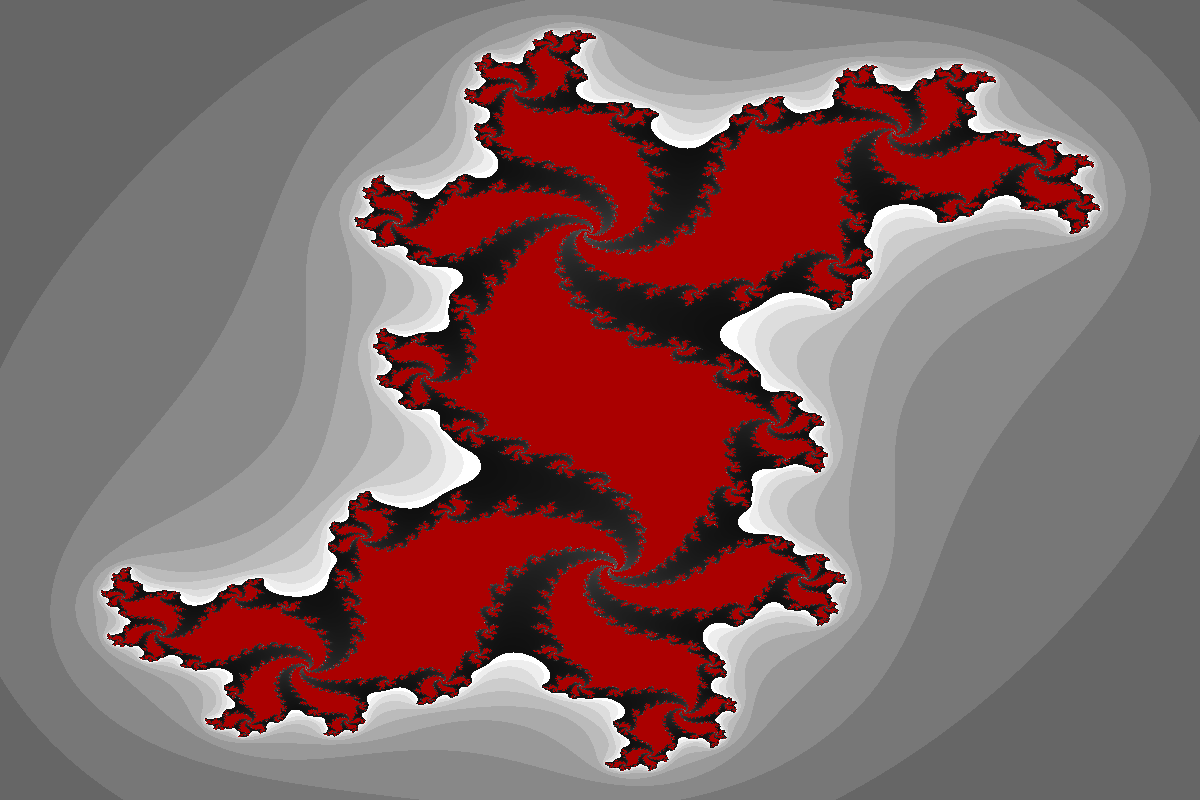
\includegraphics[scale= 0.23]{images/0305}
    \caption{Résultat \(c = 0.3 + i0.5\)}
\end{figure}

Pour \(c = -0.85 + i0.2\):

\begin{figure}[h]
    \centering
    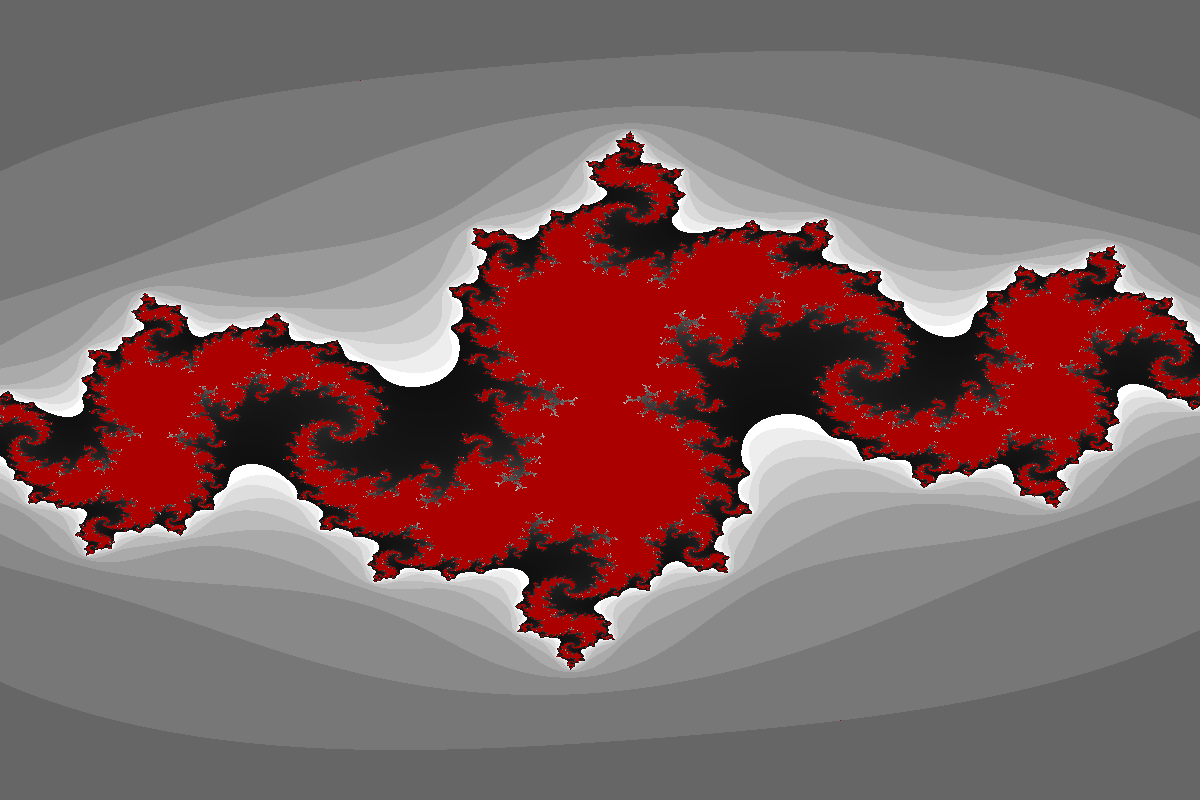
\includegraphics[scale= 0.23]{images/08502}
    \caption{Résultat \(c = -0.85 + i0.2\)}
\end{figure}

\end{document}
